
\documentclass[12pt]{article}
\usepackage[english]{babel}
\usepackage[utf8x]{inputenc}
\usepackage{amsmath}
\usepackage{etoolbox}
\usepackage{changepage}
\usepackage{titlesec}
\usepackage[parfill]{parskip}
\usepackage[margin=1in]{geometry}
\usepackage{times}
\usepackage[numbers,super]{natbib}
\usepackage{enumitem} %get rid of spaces in listened

\usepackage{hyperref}
\hypersetup{%
    colorlinks=true, 
    citecolor=black,
    linkcolor=blue,
    urlcolor =cyan } 

% For the images and graphics
\usepackage{subfig} % For subfigures in floats
\usepackage[section]{placeins}
\makeatletter
 \@ifpackageloaded{tex4ht}{%
\usepackage[dvips]{color,graphicx}
    \usepackage[tex4ht]{hyperref}
    }{%
      \usepackage[pdftex]{graphicx}
      \usepackage{hyperref}
          }
\makeatother
\graphicspath{ {/Users/omojumiller/mycode/MachineLearningNanoDegree/Machine-Learning-Project/studentIntervention} } %Path to images


% For cutesy tables
\usepackage{multirow}
\usepackage[table]{xcolor}
\usepackage{longtable}
\usepackage{array}
\usepackage{booktabs} % To draw thick lines in table.
\usepackage{tablefootnote} % To allow footnotes in table.
\newcommand{\nextitem}{\par\hspace {\labelsep} \textendash \hspace {\labelsep}} % For list inside table cell

\newcommand{\HRule}{\rule{\linewidth}{0.5mm}}


 % For text right arrow in chapter 1
 \usepackage{textcomp}
 
 % For highlighted paragraphs
\usepackage{xcolor}
\usepackage{tcolorbox}

% For listing code

% Default fixed font does not support bold face
\DeclareFixedFont{\ttb}{T1}{txtt}{bx}{n}{10} % for bold 
\DeclareFixedFont{\ttm}{T1}{txtt}{m}{n}{10}  % for normal
% Custom colors
\usepackage{color}
\definecolor{deepblue}{rgb}{0,0,0.5}
\definecolor{deepred}{rgb}{0.6,0,0}
\definecolor{deepgreen}{rgb}{0,0.5,0}


\usepackage{listings}


 % Python style for highlighting
\newcommand\pythonstyle{\lstset{
language=Python,
basicstyle=\ttm,
otherkeywords={self},             % Add keywords here
keywordstyle=\ttb\color{deepblue},
emph={MyClass,__init__},          % Custom highlighting
emphstyle=\ttb\color{deepred},    % Custom highlighting style
stringstyle=\color{deepgreen},
frame=tb,                         % Any extra options here
showstringspaces=false            % 
}}


% Python environment
\lstnewenvironment{python}[1][]
{
    \pythonstyle
    \lstset{#1}
}
{}

% Python for external files
\newcommand\pythonexternal[2][]{{
\pythonstyle
\lstinputlisting[#1]{#2}}}

% Python for inline
\newcommand\pythoninline[1]{{\pythonstyle\lstinline!#1!}}

% vector
\renewcommand{\vec}[1]{\mathbf{#1}}

%----------------------------------------------------------------------------------------
%  TITLE SECTION
%----------------------------------------------------------------------------------------
\title{\large \textbf{Building a Student Intervention System: An Udacity Nanodegree ML Project}} % using \large makes the title approximately 14 pt.
% Author info isn't included for the Annual Conference but some regional conferences might request it.
\author{Omoju Miller}
%\author{\normalsize Author Name\\
%\normalsize email@example.com\\
%\normalsize Name of Your Department\\\
%\normalsize Your Institution Name}
\date{\today} % This leaves the date blank.

\makeatletter % This gets the margins for the title set.
\patchcmd{\@maketitle}{\begin{center}}{\begin{adjustwidth}{0.5in}{0.5in}\begin{center}}{}{}
\patchcmd{\@maketitle}{\end{center}}{\end{center}\end{adjustwidth}}{}{}
\makeatother

\begin{document}
\raggedright
\maketitle
\thispagestyle{empty}
\pagestyle{empty}



%----------------------------------------------------------------------------------------
%  PAPER CONTENTS
%----------------------------------------------------------------------------------------
\section*{Introduction}
Your goal is to identify students who might need early intervention - which type of supervised machine learning problem is this, classification or regression? Why?

\begin{itemize}[noitemsep,nolistsep]
\item 
This task sounds like a problem that would be best suited for a classification algorithm. The inherent task is to develop learners that can "predicting a category." If we look at the problem from another perspective, we can consider the student data available as a ``labeled'' dataset. We have features that we can use to determine who has succeeded in the class versus who has not. For that insight, we could use `\pythoninline{passed}' column as our class label. Therefore, this is a binary classification problem for predicting discrete labels that a student might belong to.
\end{itemize}


\section*{Models}
For the student intervention challenge, three supervised learning algorithms have been selected as appropriate learners for the task. The algorithms are as follows:
\begin{enumerate}[noitemsep,nolistsep]
\item Decision Tree Classifier
\item Random Forest Classifier
\item Support Vector Machines
\end{enumerate}



\subsection*{Training and Evaluating Models: Required:}
\begin{itemize} 

\item Please give some general applications (industry applications, what are they?) of Decision Trees.
Cheap time complexity is a good reason for choosing to explore this model, but you may want to choose a reason based on what you know about the dataset.
\item Please give a general application (or industry application) of Random Forest Classifier.
\item The question states "Given what you know about the data so far, why did you choose this model to apply?" Your justification of choice for Random Forests should be based on an attribute of the dataset, so please update it.
\item Well done giving information about SVMs. You might want to elaborate on the general applications (or industry applications) of SVMs.
\end{itemize}

%-------------------------------DECISION TREE CLASSIFIER----------------------------------%

\subsection*{Decision Tree Classifier}
\begin{itemize} 
\item What is the theoretical $O(n)$ time \& space complexity in terms of input size?\\ 
The theoretical time \& space complexity of decision trees classifiers as implemented in sci-kit learn package is:
\begin{itemize}[noitemsep,nolistsep]
\item Best Case: $\Theta(pN\log^2 N)$ 
\item Worst Case: $O(pN^2\log N)$
\item Average Case: $\Theta(pN\log^2 N)$
\end{itemize}
Where $N$ denotes the number of samples, and $p$ the number of input variables. \footnote{Complexity analysis gotten from Louppe, Gilles PhD dissertation \textit{Understanding Random Forests: From Theory to Practice}, 2014.}

\item What are the general applications of this model?\\
The decision tree algorithm is usually applied to classification and regression problems.\\
What are its strengths and weaknesses?\\  
       \begin{itemize}
       \item Strengths of decision trees:
              \begin{itemize}[noitemsep,nolistsep]
                     \item Very intuitive. You can look at the results and understand it. 
                     \item Requires little data preparation. 
                     \item The cost of using the tree (i.e., predicting data) is logarithmic in the number of data points used to train the tree. In average case the cost of training $ O(pN\log^2 N)$
                     \item Able to handle both numerical and categorical data.
                     \item Very robust. Performs well even if its assumptions are somewhat violated by the true model from which the data were generated.
              \end{itemize}
       \item Weaknesses of decision trees:
              \begin{itemize}[noitemsep,nolistsep]
                     \item Decision-tree learners can create over-complex trees that do not generalize the data well. They are prone to over-fitting especially in the case of data with lots of features.
                     \item Decision trees can be unstable because small variations in the data might result in a completely different tree being generated. 
                     \item The problem of learning an optimal decision tree is known to be NP-complete under several aspects of optimality and even for simple concepts. 
                     \item There are concepts that are hard to learn because decision trees do not express them easily, such as XOR, parity or multiplexer problems.
                     \item Decision tree learners create biased trees if some classes dominate. 
              \end{itemize}
       \end{itemize}


\item Given what you know about the data so far, why did you choose this model to apply?\\
The decision tree classifier was chosen because of its ease of use and its relatively cheap time complexity.\\
Another \textit{major} reason why the decision tree classifier was selected was its interpretability. For this problem domain, it isn't just satisfactory to identify students that need intervention, what learning researchers ultimately want is to gain \textit{insights} into the nature of learning, and the social factors that lead to certain outcomes for at-risk students. A decision tree learner, with its ability to graphically plot out the tree becomes a research tool in the hands of learning scientist. Consequently, this can help the school board of supervisors build better solutions for those students which well executed could potentially reduce the costs associated with remediating failed students.
\end{itemize} 




%-----------------------------RANDOM FOREST CLASSIFIER---------------------------------------%

\subsection*{Random Forest Classifier}
\begin{itemize} 
\item What is the theoretical $O(n)$ time \& space complexity in terms of input size?\\
The theoretical time \& space complexity for building a complete unpruned decision tree is:
\begin{itemize}[noitemsep,nolistsep]
\item Best Case: $\Theta(MK\widetilde{N}\log^2 \widetilde{N})$ 
\item Worst Case: $O(MK\widetilde{N}^2\log \widetilde{N})$ 
\item Average Case: $\Theta(MK\widetilde{N}\log^2 \widetilde{N})$
\end{itemize}
Where $M$ denotes number of randomized trees, $N$ the number of samples, and $K$ the number of variables randomly drawn at each node. $\widetilde{N} = 0.632 N$, due to the fact that bootstrap samples draw, on average, $63.2\%$ of unique samples. 
\footnote{Complexity analysis gotten from Louppe, Gilles PhD dissertation \textit{Understanding Random Forests: From Theory to Practice}, 2014.}

\item What are the general applications of this model?\\
Ensemble learners are used in supervised learning. The goal of the random forest classifier is to combine the results of multiple classifiers, yielding an ensemble of decision trees. The prediction of the classifier is the averaged prediction of the individual classifiers.

\item What are its strengths and weaknesses?\\
\begin{itemize}[noitemsep,nolistsep]
       \item Strenghts of SVMs:
              \begin{itemize}[noitemsep,nolistsep]
                     \item Considered one of the best off-the-shelf learning algorithm, requires almost no tuning. 
                     \item Fast to train because algorithm lends itself well to parallelization
                     \item Flexible, can be used with large number of attributes, small or large datasets
                     \item Good control of bias and variance because of the averaging and randomization which leads to better performance.
              \end{itemize}
       \item Weaknesses of decision trees:
              \begin{itemize}[noitemsep,nolistsep]
                     \item Loss of interpretability as compared to decision trees give.
              \end{itemize}
       \end{itemize}


\item Given what you know about the data so far, why did you choose this model to apply?\\
This learners was chosen as a means of reducing the effects of overfitting of decision trees.
\end{itemize} 



%-------------------------------------------S V M -----------------------------------------%

\subsection*{Support Vector Machine (SVMs)}
\begin{itemize}
\item What is the theoretical $O(n)$ time \& space complexity in terms of input size?\\
The theoretical time \& space complexity of SVMs is:
\begin{itemize}[noitemsep,nolistsep]
\item Best Case: $\Theta(pN^2)$ 
\item Worst Case: $O(pN^3)$
\item Average Case: $\Theta(pN^2)$
\end{itemize}
Where $N$ denotes the number of samples, and $p$ the number of input variables. 
It can be a costly algorithm since the compute and storage requirements increase rapidly with the number of training vectors. Even though the algorithm spends more time in the training, however, it achieves better $ F_1$ score for prediction – thus it is more accurate.

\item What are the general applications of this model?\\ 
SVMs are an algorithm used for classification, regression and outlier detection.\\
What are its strengths and weaknesses?
\begin{itemize}
       \item Strenghts of SVMs:
              \begin{itemize}[noitemsep,nolistsep]
                     \item Versatile: utilizes \textbf{kernel} transformation and several functional forms so that what was once non-linearly separable now becomes linearly separable.
                     \item Effective in high dimensional spaces.
                     \item Still effective in cases where number of dimensions is greater than the number of samples.
                     \item Uses a subset of training points in the decision function (called support vectors), so it is also memory efficient.
              \end{itemize}
       \item Weaknesses of decision trees:
              \begin{itemize}[noitemsep,nolistsep]
                     \item If the number of features is much greater than the number of samples, the method is likely to give poor performances.
                     \item SVMs do not directly provide probability estimates, these are calculated using an expensive five-fold cross-validation.
                     \item SVM is a binary classifier. To do a multi-class classification, only pair-wise classifications can be used (one class against all others, for all classes).
              \end{itemize}
       \end{itemize}

\item Given what you know about the data so far, why did you choose this model to apply?\\
The general approach is to try a few different algorithms for each problem. Sci-kit learn provides a guide to choosing estimators. Based on the guide, and our task satisfying the following criteria: {100K \textgreater samples \textgreater 50, goal of predicting a category \& availability of labeled data}, a linear SVC was selected. 
\end{itemize}

%----------------------------------------------------------------------------------------

\section*{Choosing the Best Model}

\subsection*{Required:}
\begin{itemize} 

\item Please thoroughly compare the F1 scores and computation costs of each model with each other model.
Well done using accuracy to choose SVMs, however. Please make your comparison more thorough, and include Decision Trees in your comparison.
\end{itemize}

\paragraph{\textbf{Question}} Based on the experiments you performed earlier, in 1-2 paragraphs explain to the board of supervisors what single model you chose as the best model. Which model is generally the most appropriate based on the available data, limited resources, cost, and performance?

\begin{figure}[!htbp]
  \centering
    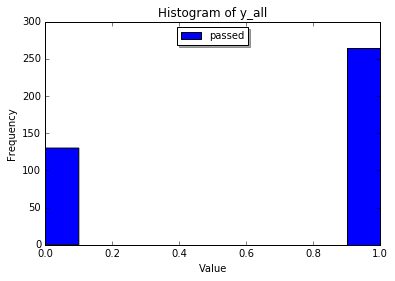
\includegraphics[width=0.5\textwidth]{images/y_all}
  %
\caption{\textbf{Values of `passed' column} \textit{The histograms shows an unbalanced target dataset with approximately 125 values of (0) and over 250 values of (1).}}
\label{y_all}
\end{figure}


\paragraph{\textbf{Answer}} For the problem of identifying students that need intervention, I would advice the board of supervisors to go with a \textbf{Support Vector Machine}. First, it is a relatively fast algorithm to train and predict. 
Second, as we can see from figure \ref{y_all}, the dataset is quite unbalanced (number of passed students $>>$ number of failed students) a relatively small. The SVM algorithm is able to handle this better than the other two models. 

While its marginally slower in prediction than Random Forest classifier with a prediction time of 0.001 versus 0.006 as can be seen from tables \ref{randomForestClassifierTable} and \ref{svmTable}. The difference of negligible and SVM makes up for what it loses in speed with improvement in accuracy.


\paragraph{\textbf{Question}} In 1-2 paragraphs explain to the board of supervisors in layman's terms how the final model chosen is supposed to work (for example if you chose a Decision Tree or Support Vector Machine, how does it make a prediction).

\paragraph{\textbf{Answer}} A Support Vector Machine is a class of discriminatory algorithms. The goal is to try and correctly classify a dataset into separate classes. Subject to that constraint, an SVM  picks a decision boundary that separates the classes by maximizing the distance to the nearest points in either classes. These points are a subset of the dataset and are called support vectors. 


\begin{figure}[!hbtp]
\centering
    \subfloat[Features in two dimensional space.]{%
    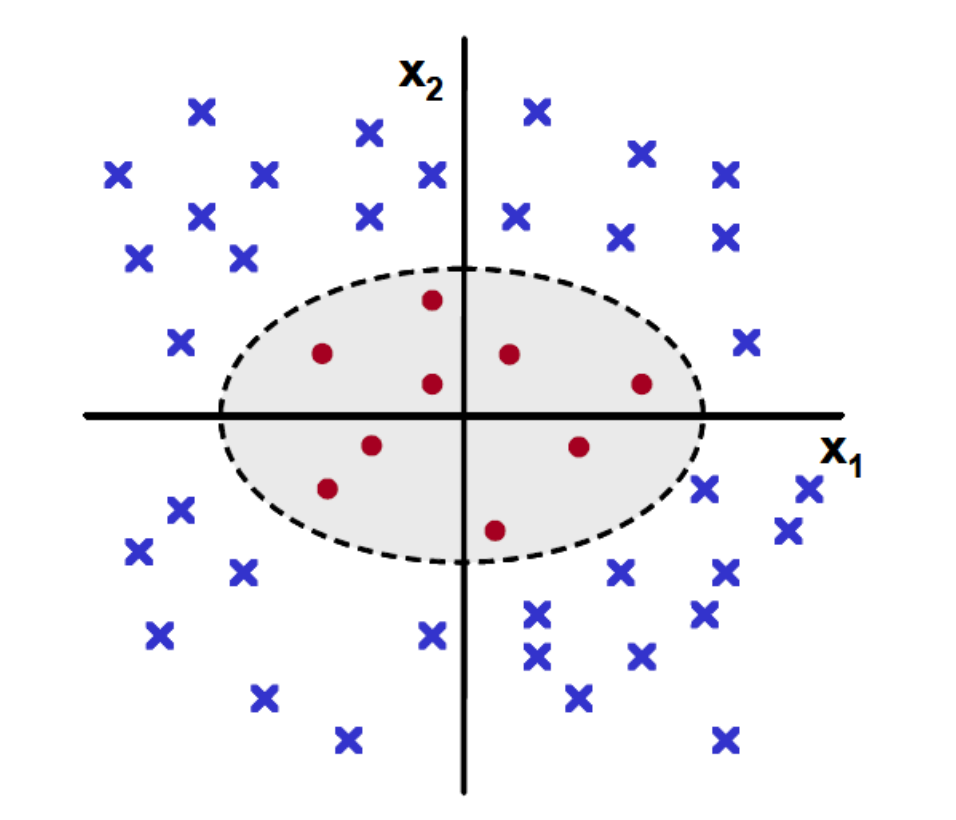
\includegraphics[width=0.5\textwidth]{images/SVMNonlinear1}
    \label{SVMNonlinear1}}
    \subfloat[Features projected in three dimensional space.]{%
    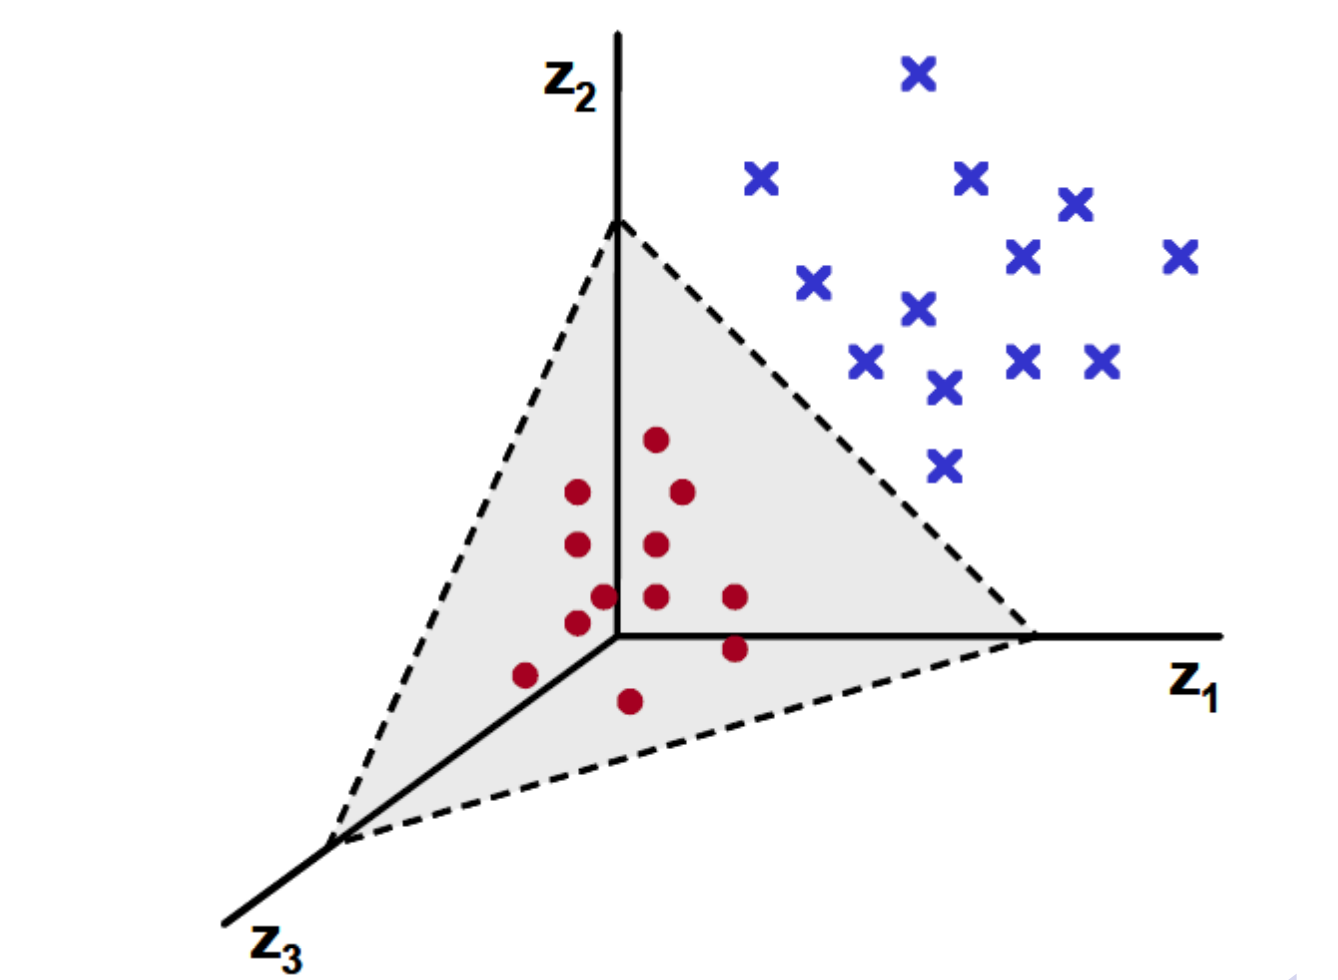
\includegraphics[width=0.5\textwidth]{images/SVMNonlinear2}
    \label{SVMNonlinear2}}
    \caption{\textbf{Kernel trick.} \textit{Figure (a) $\vec{x} = \{x_1,x_2\}$. Figure (b) $\vec{z}$ by $\vec{x} = \{x_1,x_2\} \longrightarrow \vec{z} = \{x_1^2, \sqrt2x_1x_2, x_2^2 \}$. By mapping the data from two dimensions to three dimension, the data now becomes linearly separable in the new representation.}}
\end{figure}

The most interesting thing about SVMs is what is know as the \textit{kernel} trick. This procedure make linear models work in nonlinear settings by mapping the data into higher dimensions where we can see the linear behavior. For example, the figure in \ref{SVMNonlinear1} shows a data in two-dimensional space where it is evident we will not be able to find a decision boundary that separates it into two classes. Using a kernel, the features are projected into a three dimension space as is shown in figure \ref{SVMNonlinear2} where we can find a hyperplane that will linearly separate the data into two classes. This aspect of SVMs is what makes them really robust.

An SVM does prediction on the data by classifying the test dataset based on the decision boundary it ``fitted'' during its training phase. There are several evaluation metrics that let you determine the accuracy of the algorithm.


\paragraph{\textbf{Question}} Fine-tune the model. What is the model's final F1 score?

\setlength{\extrarowheight}{1.5pt}
\begin{table}[!htbp]
\caption{Result of tuning with \textbf{GridSearchCV}} %title of the table
\centering % centering table
\begin{tabular}{|p{4cm}||p{4cm}|} % creating four columns
\hline % inserts single-line
& GridSearchCV\\[0.5ex]
\hline % inserts single-line

F1 score for training set     &1.000\\
F1 score for test set         &0.803\\
\hline % inserts single-line
\end{tabular}
\label{tunedGridSearch}
\end{table}








%-------------------------------------------T A B L E S-----------------------------------------%

\section*{Tables}

\setlength{\extrarowheight}{1.5pt}
\begin{table}[!htbp]
\caption{Result of training with a \textbf{DecisionTreeClassifier}} %title of the table
\centering % centering table
\begin{tabular}{|p{6cm}|p{1.5cm}|p{1.5cm}|p{1.5cm}|} % creating four columns
\hline % inserts single-line
& \multicolumn{3}{c|}{Training set size}\\[5pt]
\cline{2-4} 
& 100 & 200 & 300\\[0.5ex]
\hline % inserts single-line

Training time (secs)          &0.001&0.001&0.002\\
Prediction time (secs)        &0.000&0.000&0.000\\
F1 score for training set     &1.000&1.000&1.000\\
F1 score for test set         &0.746&0.649&0.720\\

\hline % inserts single-line
\end{tabular}
\label{decisionTreeTable}
\end{table}

\setlength{\extrarowheight}{1.5pt}
\begin{table}[!htbp]
\caption{Result of training with a \textbf{Random Forest Classifier}} %title of the table
\centering % centering table
\begin{tabular}{|p{6cm}|p{1.5cm}|p{1.5cm}|p{1.5cm}|} % creating four columns
\hline % inserts single-line
& \multicolumn{3}{c|}{Training set size}\\[5pt]
\cline{2-4} 
& 100 & 200 & 300\\[0.5ex]
\hline % inserts single-line

Training time (secs)          &0.031&0.030&0.026\\
Prediction time (secs)        &0.001&0.001&0.001\\
F1 score for training set     &0.994&1.000&0.988\\
F1 score for test set         &0.701&0.744&0.713\\
\hline % inserts single-line
\end{tabular}
\label{randomForestClassifierTable}
\end{table}


\setlength{\extrarowheight}{1.5pt}
\begin{table}[!htbp]
\caption{Result of training with a \textbf{SVMs}} %title of the table
\centering % centering table
\begin{tabular}{|p{6cm}|p{1.5cm}|p{1.5cm}|p{1.5cm}|} % creating four columns
\hline % inserts single-line
& \multicolumn{3}{c|}{Training set size}\\[5pt]
\cline{2-4} 
& 100 & 200 & 300\\[0.5ex]
\hline % inserts single-line

Training time (secs)          &0.001&0.003&0.006\\
Prediction time (secs)        &0.001&0.001&0.002\\
F1 score for training set     &0.886&0.879&0.877\\
F1 score for test set         &0.782&0.754&0.752\\
\hline % inserts single-line
\end{tabular}
\label{svmTable}
\end{table}


\end{document}  